\documentclass[journal]{IEEEtran}
\usepackage{amsmath,amsfonts}
\usepackage{algorithmic}
\usepackage{algorithm}
\usepackage{array}
\usepackage[caption=false,font=normalsize,labelfont=sf,textfont=sf]{subfig}
\usepackage{textcomp}
\usepackage{stfloats}
\usepackage{url}
\usepackage{verbatim}
\usepackage{graphicx}
\usepackage{cite}
\usepackage[spanish]{babel}
\usepackage{pgfplots}
\DeclareUnicodeCharacter{2212}{−}
\usepgfplotslibrary{groupplots,dateplot}
\usetikzlibrary{patterns,shapes.arrows}
\pgfplotsset{compat=newest}

\hyphenation{op-tical net-works semi-conduc-tor IEEE-Xplore}
% updated with editorial comments 8/9/2021
\begin{document}

\title{Evaluación de algoritmos de búsqueda para la resolución del problema de las jarras}

\author{\IEEEauthorblockN{E. E. Reza Garduño, W. Esquivel Diaz, G. Salgado Agreda}}

\maketitle

\begin{abstract}
  El problema de las jarras es un clásico ejemplo de un problema matemático y lógico que requiere de habilidades de razonamiento y pensamiento creativo para resolverlo. Resolver este problema puede tener aplicaciones prácticas en el campo de la inteligencia artificial, la optimización y la resolución de problemas, lo que lo hace un tema de gran interés en la investigación y el aprendizaje. En esta ocasion se propone la implementación de algoritmos de búsqueda para resolver dicho problema.
\end{abstract}

\section{Introducción}
Sean dos jarras de capacidad $x$ y $y$ respectivamente, y un líquido de capacidad infinita. Se desea obtener $z$ litros de líquido en una de las jarras. ¿Cómo se puede lograr esto?. 

El enunciado anterior es la descripción del problema de las jarras, un problema clásico que se puede encontrar en libros de matemáticas, en la literatura de inteligencia artificial y en la web. El problema de las jarras es un problema de búsqueda en el que se busca una solución a un problema a partir de un estado inicial. En este caso, el estado inicial es el estado en el que se encuentran las jarras, y el estado final es el estado en el que se encuentran las jarras después de haber realizado las operaciones necesarias para obtener $z$ litros de líquido en una de las jarras.

Para lograr alcanzar $z$ se consideran algunas restricciones:
\begin{itemize}
  \item No se puede medir el líquido que se encuentra en las jarras, solo se puede saber si la jarra está vacía o llena, asi como la cantidad restante de alguna operación.
  \item Solo se pueden realizar las siguientes operaciones:
  \begin{itemize}
    \item Llenar la jarra de $x$ litros.
    \item Llenar la jarra de $y$ litros.
    \item Vaciar la jarra de $x$ litros.
    \item Vaciar la jarra de $y$ litros.
    \item Llenar la jarra de $x$ litros desde la jarra de $y$ litros.
    \item Llenar la jarra de $y$ litros desde la jarra de $x$ litros.
  \end{itemize}
\end{itemize}

Viendo el problema, se puede obtener la solución rápida y fácilmente, sin embargo, para el caso de que se desee obtener la solución de manera automática, la solución para la computadora no es tan evidente.
Después de todo, la computadora no puede pensar como un humano, por lo que se requiere de un algoritmo que le indique a la computadora qué operaciones realizar para llegar a la solución.
Pero ahora tenemos otro problema, ¿cómo se puede implementar un algoritmo que le indique a la computadora qué operaciones realizar para llegar a la solución?. Es en este punto cuando aparecen los algoritmos de búsqueda, que son algoritmos que permiten encontrar una solución a un problema a partir de un estado inicial. Aun así, cabe mencionar que este problema puede ser resuelto de muchas otras maneras, pero nos enfocaremos en los algoritmos de búsqueda.

Considerado solo dos jarras, la complejidad de este problema se puede aproximar como $O(m \cdot n)$, donde $m$ y $n$ son las capacidades de cada jarra. La cantidad de estados aumenta como se muestra a continuación:

\begin{figure}[h]
  \centering
  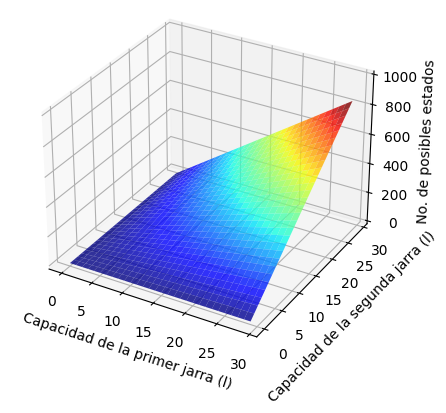
\includegraphics[width=0.45\textwidth]{figures/estados.png}
  \centering
  \caption{Cantidad de estados}
  \label{fig:estados}  
\end{figure}

Es importante recordar que no todos los posibles estados son alacanzables, por lo que la cantidad de estados alcanzables es menor a la cantidad de estados totales.

En este trabajo, usaremos algunos algorimos de búsqueda para resolver el problema de las jarras, comparando los resultados obtenidos entre si, a fin de determinar cuales son los algoritmos más eficientes para resolver este problema.
\section{Trabajos relacionados}

\section{Enfoque}
Formulamos el problema de las jarras como un árbol de búsqueda, donde cada nodo representa un estado, y cada arista representa una operación. Como muchos de este tipo de problemas, varias veces una operación puede llevar a un estado que ya se ha visitado, por lo que se debe de tener cuidado de no repetir estados.
Para lograr eso ultimo, existirá una lista de estados visitados, y cada vez que se visite un estado, se revisará si ya se ha visitado, en caso de que ya se haya visitado, se ignorará el estado, evitando así desarrollos infinitos.

Para cada nodo se podrán desarrollar hasta 6 hijos, uno para cada operación, a consideración de que la operación sea posible de realizar. Por ejemplo, si la jarra de $x$ litros está llena, no se podrá realizar la operación de llenar la jarra de $x$ litros, ya que la jarra ya está llena. Por otro lado, si la jarra de $y$ litros está vacía, no se podrá realizar la operación de vaciar la jarra de $y$ litros, ya que la jarra ya está vacía. Para estos casos, se ignorará la operación, y se desarrollará el siguiente hijo.
Y siempre teniendo en consideración que el estado final deseado puede no ser alcanzable.



\section{Experimentos}

\section{Conclusion}
The conclusion goes here.

\section{Trabajos futuros}

\section{Participación de los autores}
\begin{itemize}
  \item E. E. Reza Garduño: 0\%
  \item W. Esquivel Diaz: 0\%
  \item G. Salgado Agreda: 0\%
\end{itemize}

\begin{thebibliography}{1}
  \bibliographystyle{IEEEtran}

  \bibitem{ref1}
  {\it{Mathematics Into Type}}. American Mathematical Society. [Online]. Available: https://www.ams.org/arc/styleguide/mit-2.pdf

  \bibitem{ref2}
  T. W. Chaundy, P. R. Barrett and C. Batey, {\it{The Printing of Mathematics}}. London, U.K., Oxford Univ. Press, 1954.

  \bibitem{ref3}
  F. Mittelbach and M. Goossens, {\it{The \LaTeX Companion}}, 2nd ed. Boston, MA, USA: Pearson, 2004.

  \bibitem{ref4}
  G. Gr\"atzer, {\it{More Math Into LaTeX}}, New York, NY, USA: Springer, 2007.

  \bibitem{ref5}M. Letourneau and J. W. Sharp, {\it{AMS-StyleGuide-online.pdf,}} American Mathematical Society, Providence, RI, USA, [Online]. Available: http://www.ams.org/arc/styleguide/index.html

  \bibitem{ref6}
  H. Sira-Ramirez, ``On the sliding mode control of nonlinear systems,'' \textit{Syst. Control Lett.}, vol. 19, pp. 303--312, 1992.

  \bibitem{ref7}
  A. Levant, ``Exact differentiation of signals with unbounded higher derivatives,''  in \textit{Proc. 45th IEEE Conf. Decis.
    Control}, San Diego, CA, USA, 2006, pp. 5585--5590. DOI: 10.1109/CDC.2006.377165.

  \bibitem{ref8}
  M. Fliess, C. Join, and H. Sira-Ramirez, ``Non-linear estimation is easy,'' \textit{Int. J. Model., Ident. Control}, vol. 4, no. 1, pp. 12--27, 2008.

  \bibitem{ref9}
  R. Ortega, A. Astolfi, G. Bastin, and H. Rodriguez, ``Stabilization of food-chain systems using a port-controlled Hamiltonian description,'' in \textit{Proc. Amer. Control Conf.}, Chicago, IL, USA,
  2000, pp. 2245--2249.

\end{thebibliography}

\end{document}


